\chapter{Enquisa}
\label{chap:encuesta}

%%%%%%%%%%%%%%%%%%%%%%%%%%%%%%%%%%%%%%%%%%%%%%%%%%%%%%%%%%%%%%%%%%%%%%%%%%%%%%%%
% Objetivo: Lista de términos utilizados en el documento,                      %
%           junto con sus respectivos significados.                            %
%%%%%%%%%%%%%%%%%%%%%%%%%%%%%%%%%%%%%%%%%%%%%%%%%%%%%%%%%%%%%%%%%%%%%%%%%%%%%%%%

\lettrine{N}{este} apéndice exponse a enquisa mediante a que se levou a cabo o
estudio de viabilidade.

\section{Resultados}

A continuación expóñense os resultados obtidos.

\begin{figure}
 \centering
 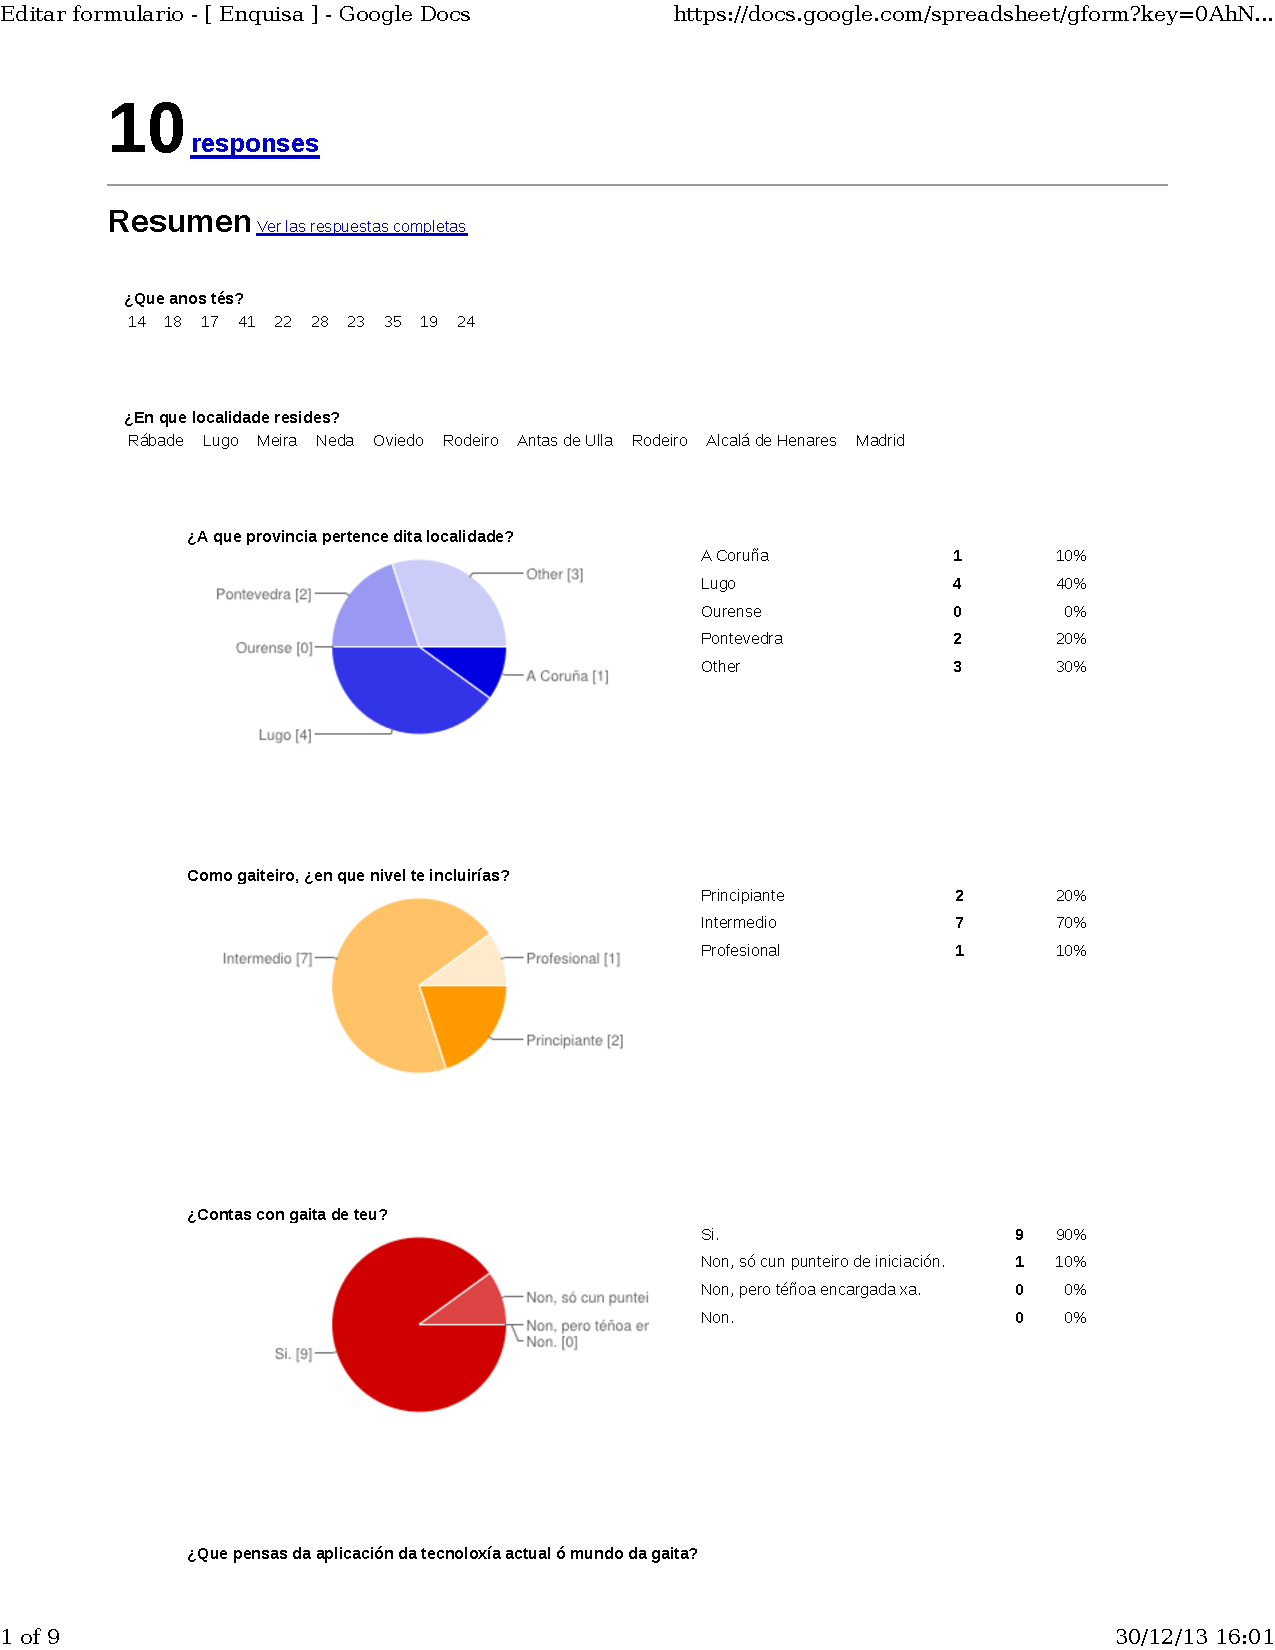
\includegraphics[scale=0.7,page=1,keepaspectratio=true,clip,trim=0cm 0.5cm 0cm 0.5cm]{./imagenes/enquisa.pdf}
 % enquisa.pdf: 612x792 pixel, 72dpi, 21.59x27.94 cm, bb=0 0 612 792
 \caption{Resultados da enquisa (p. 1).}
 \label{figura:ResultadosEnquisa1}
\end{figure}

\begin{figure}
 \centering
 \includegraphics[scale=0.7,page=2,keepaspectratio=true,clip,trim=0cm 0.5cm 0cm 0.5cm]{./imagenes/enquisa.pdf}
 % enquisa.pdf: 612x792 pixel, 72dpi, 21.59x27.94 cm, bb=0 0 612 792
 \caption{Resultados da enquisa (p. 2).}
 \label{figura:ResultadosEnquisa2}
\end{figure}

\begin{figure}
 \centering
 \includegraphics[scale=0.7,page=3,keepaspectratio=true,clip,trim=0cm 22cm 0cm 0.5cm]{./imagenes/enquisa.pdf}
 % enquisa.pdf: 612x792 pixel, 72dpi, 21.59x27.94 cm, bb=0 0 612 792
 \caption{Resultados da enquisa (p. 3).}
 \label{figura:ResultadosEnquisa3}
\end{figure}

\begin{figure}
 \centering
 \includegraphics[scale=0.7,page=4,keepaspectratio=true,clip,trim=0cm 0.5cm 0cm 0.5cm]{./imagenes/enquisa.pdf}
 % enquisa.pdf: 612x792 pixel, 72dpi, 21.59x27.94 cm, bb=0 0 612 792
 \caption{Resultados da enquisa (p. 4).}
 \label{figura:ResultadosEnquisa4}
\end{figure}

\begin{figure}
 \centering
 \includegraphics[scale=0.7,page=5,keepaspectratio=true,clip,trim=0cm 0.5cm 0cm 0.5cm]{./imagenes/enquisa.pdf}
 % enquisa.pdf: 612x792 pixel, 72dpi, 21.59x27.94 cm, bb=0 0 612 792
 \caption{Resultados da enquisa (p. 5).}
 \label{figura:ResultadosEnquisa5}
\end{figure}

\begin{figure}
 \centering
 \includegraphics[scale=0.7,page=6,keepaspectratio=true,clip,trim=0cm 0.5cm 0cm 0.5cm]{./imagenes/enquisa.pdf}
 % enquisa.pdf: 612x792 pixel, 72dpi, 21.59x27.94 cm, bb=0 0 612 792
 \caption{Resultados da enquisa (p. 6).}
 \label{figura:ResultadosEnquisa6}
\end{figure}

\begin{figure}
 \centering
 \includegraphics[scale=0.7,page=7,keepaspectratio=true,clip,trim=0cm 0.5cm 0cm 0.5cm]{./imagenes/enquisa.pdf}
 % enquisa.pdf: 612x792 pixel, 72dpi, 21.59x27.94 cm, bb=0 0 612 792
 \caption{Resultados da enquisa (p. 7).}
 \label{figura:ResultadosEnquisa7}
\end{figure}

\begin{figure}
 \centering
 \includegraphics[scale=0.7,page=8,keepaspectratio=true,clip,trim=0cm 0.5cm 0cm 0.5cm]{./imagenes/enquisa.pdf}
 % enquisa.pdf: 612x792 pixel, 72dpi, 21.59x27.94 cm, bb=0 0 612 792
 \caption{Resultados da enquisa (p. 8).}
 \label{figura:ResultadosEnquisa8}
\end{figure}

\begin{figure}
 \centering
 \includegraphics[scale=0.7,page=9,keepaspectratio=true,clip,trim=0cm 22cm 0cm 0cm]{./imagenes/enquisa.pdf}
 % enquisa.pdf: 612x792 pixel, 72dpi, 21.59x27.94 cm, bb=0 0 612 792
 \caption{Resultados da enquisa (p. 9).}
 \label{figura:ResultadosEnquisa9}
\end{figure}